\documentclass[a4paper,10pt]{article}

%%Packages	%%%	%%%	%%%	%%%	%%%	%%%	%%%
\usepackage{amsmath,framed}
\usepackage[utf8]{inputenc} 	
\usepackage{listings}
\usepackage{xcolor}
\usepackage{graphicx}
\usepackage{placeins}

%%Settings	%%%	%%%	%%%	%%%	%%%	%%%	%%%
\renewcommand{\d}{\text{d}}
\newcommand{\e}{\text{e}}
\newcommand{\ve}{\mathbf}
\newcommand\numb{\addtocounter{equation}{1}\tag{\theequation}}

\setlength\fboxsep{1.2mm}
\setlength\fboxrule{0.5mm}


%%Margins	%%%	%%%	%%%	%%%	%%%	%%%	%%%
\usepackage{geometry}
\geometry{
  a4paper,
  left=35mm,
  right=35mm,
  top=25mm,
  bottom=25mm,
}

%%Header & Footer	%%%	%%%	%%%	%%%	%%%	%%%
\usepackage{fancyhdr}
\pagestyle{fancy}
\renewcommand{\headrulewidth}{1pt}
\rhead{Sara Danielsson, Mikael Perssson}
%8509080456 mitt persnr om vi vill ha det
\lhead{L3 DD2431}

\title{Lab 3, DD2431 Machine Learning}
\author{Sara Danielsson \\ Mikael Persson}
\begin{document}
%\maketitle

%\subsubsection*{Assignment 1}
\iffalse
Bayes Theorem is given by
\begin{align*}
  P(\alpha | D) &= \frac{P(D|\alpha)P(\alpha)}{P(D)} \Leftrightarrow \\
  \text{posterior} &= \frac{\text{likelihood}\times \text{prior}}{\text{evidence}},
\end{align*}
where $\alpha$ denote the model parameters and $D$ is the data.
\emph{Bayes Classification} uses the class posterior for a point $x^*$ belonging to a class
$k$ given by
\begin{equation*}
  P(k|x^*) = \frac{P_k(x^*|k)P(k)}{\underset{{k_i \in C}}{\sum}P_{k_i}(x^*|k_i)P(k_i)}
\end{equation*}
where $p_k(x^*|k)$ is the class conditional density, $C$ is the set of classes and $p(k)$
is the prior probability of class $k$. Assuming the density is described by a multivariat Gaussian 
we have
\begin{equation*}
  p_k(x|k) = \frac{1}{\sqrt{(2 \pi)^d \det \Sigma}}
  \e^{-\frac{1}{2}(x-\mu)\Sigma^{-1}(x - \mu)^\top}
\end{equation*}
where $x$ is a $1\times d$ row vector, and $\mu,\Sigma$ are the mean vector and 
covariance matrix respectively. Making the assumption that the data points are i.i.d. and 
maximizing the log likelihood gives the ML-estimates
\begin{align*}
  \mu_k &= \frac{1}{N_k}\sum_{i:c_i = k} x_i \\
  \Sigma_k &=
\end{align*}
\fi
\noindent
\textbf{Assignment 1}
\\
Please refer to the code for implementation of \texttt{mlParams()}.
Figure \ref{FIGas1} shows the result.




\FloatBarrier
\begin{figure}[h!]
  \center
  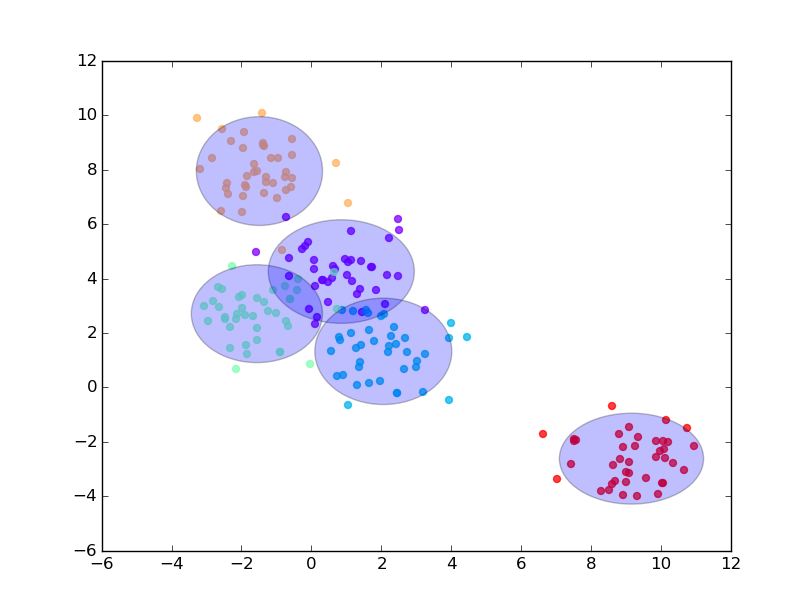
\includegraphics[width = 150mm]{figure_1.png}
  \vspace{-15mm}

  \begin{minipage}[t]{95mm}
    \caption{
      95 \% confidence intervals for data generated by \texttt{genBlobs(centers = 5)}
    }
    \label{FIGas1}
  \end{minipage}
\end{figure}

\FloatBarrier
$ $\\
\textbf{Assignment 2}
\\
Refer to code for implementations of \texttt{computePrior()} and \texttt{classifyBayes()}.



%\newpage
$ $\\
\textbf{Assignment 3}\\
The result of running \texttt{testClassifier(BayesClassifier(), dataset='iris', split=0.7)} and 
\texttt{testClassifier(BayesClassifier(), dataset='vowel', split=0.7)}
is given:
\begin{framed}
  \begin{scriptsize}
  \begin{verbatim}
  Trial: 0 Accuracy 84.4
  Trial: 10 Accuracy 95.6
  Trial: 20 Accuracy 93.3
  Trial: 30 Accuracy 86.7
  Trial: 40 Accuracy 88.9
  Trial: 50 Accuracy 91.1
  Trial: 60 Accuracy 86.7
  Trial: 70 Accuracy 91.1
  Trial: 80 Accuracy 86.7
  Trial: 90 Accuracy 91.1
  Final mean classification accuracy  89 with standard deviation 4.16
  Trial: 0 Accuracy 61
  Trial: 10 Accuracy 66.2
  Trial: 20 Accuracy 74
  Trial: 30 Accuracy 66.9
  Trial: 40 Accuracy 59.7
  Trial: 50 Accuracy 64.3
  Trial: 60 Accuracy 66.9
  Trial: 70 Accuracy 63.6
  Trial: 80 Accuracy 62.3
  Trial: 90 Accuracy 70.8
  Final mean classification accuracy  64.7 with standard deviation 4.03
  \end{verbatim}
  \end{scriptsize}
\end{framed}
\noindent
The decision boundary for the 2D-iris data is depicted in Figure \ref{FIGas2}.

\FloatBarrier
\begin{figure}[h!]
  \center
  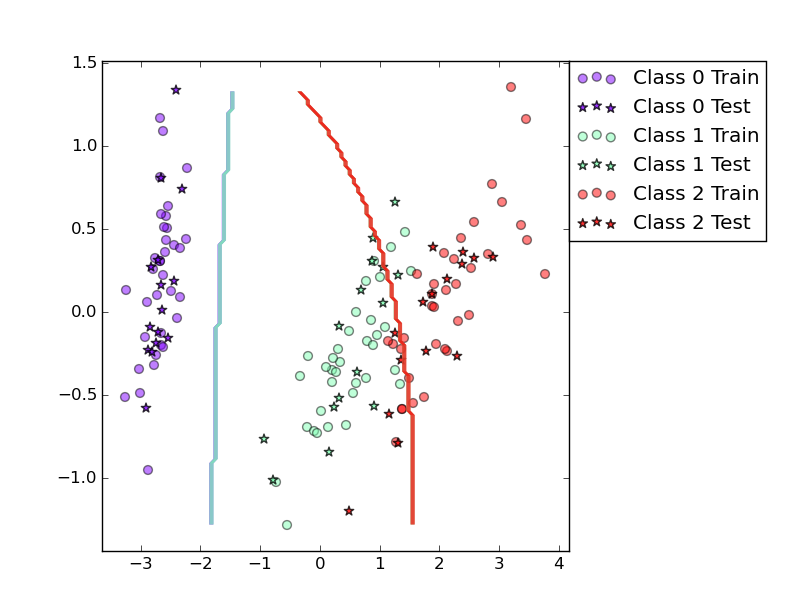
\includegraphics[width = 150mm]{figure_2.png}
  \vspace{-15mm}

  \begin{minipage}[t]{95mm}
    \caption{
      Boundary for the iris data.
    }
    \label{FIGas2}
  \end{minipage}
\end{figure}

\FloatBarrier
\noindent
Questions:
\begin{itemize}
  \item[1)] When can feature independence assumption be reasonable?
  \item[A:] When one may assume that there is no or little correlation between the 
    features. In the Iris-set one may assume that there is positive correlation
    between petal width and petal length (or sepal width \& length), c.f.
    \texttt{https://archive.ics.uci.edu/ml/datasets/Iris}.
  \item[2)] How does the decision boundary look for the iris dataset? How could one improve the
    results for this scenario by changing the classifier, or by manipulating the data?
  \item[A:] It looks like class 0 is has fairly uncorrelated features while class 1 and class 2 
    has not. One could use a ``non-naive'' Bayes classifier, i.e. where it is not 
    necissarily the case that 
    $\Sigma(m,n) = 0, \quad n \ne m$. One could possibly make non linear
    transformation of the data.
\end{itemize}
$ $\\
\textbf{Assignment 4}
\\
Refer to code for the augmented functions \texttt{mlParams()}





$ $\\
\textbf{Assignment 5}
\\
Refer to code for augmented function \texttt{computePrior()}. Also for 
implementations of \texttt{trainBoost()} and \texttt{classifyBoost()}.
The results of running 
\begin{scriptsize}
  \begin{verbatim}
  testClassifier(BoostClassifier(BayesClassifier(), T=10), dataset='iris',split=0.7)
  testClassifier(BoostClassifier(BayesClassifier(), T=10), dataset='vowel',split=0.7)
  \end{verbatim}
\end{scriptsize}
are given below.
Decision boundary for the iris data using boosting is given in Figure \ref{FIGas3}.


\newpage
\begin{framed}
  \begin{scriptsize}
  \begin{verbatim}
  Trial: 0 Accuracy 95.6
  Trial: 10 Accuracy 100
  Trial: 20 Accuracy 93.3
  Trial: 30 Accuracy 91.1
  Trial: 40 Accuracy 97.8
  Trial: 50 Accuracy 93.3
  Trial: 60 Accuracy 93.3
  Trial: 70 Accuracy 97.8
  Trial: 80 Accuracy 95.6
  Trial: 90 Accuracy 93.3
  Final mean classification accuracy  94.7 with standard deviation 2.82
  Trial: 0 Accuracy 76.6
  Trial: 10 Accuracy 86.4
  Trial: 20 Accuracy 83.1
  Trial: 30 Accuracy 80.5
  Trial: 40 Accuracy 72.7
  Trial: 50 Accuracy 76
  Trial: 60 Accuracy 81.8
  Trial: 70 Accuracy 82.5
  Trial: 80 Accuracy 79.9
  Trial: 90 Accuracy 83.1
  Final mean classification accuracy  80.2 with standard deviation 3.52
  \end{verbatim}
  \end{scriptsize}
\end{framed}
\noindent












\FloatBarrier
\begin{figure}[h!]
  \center
  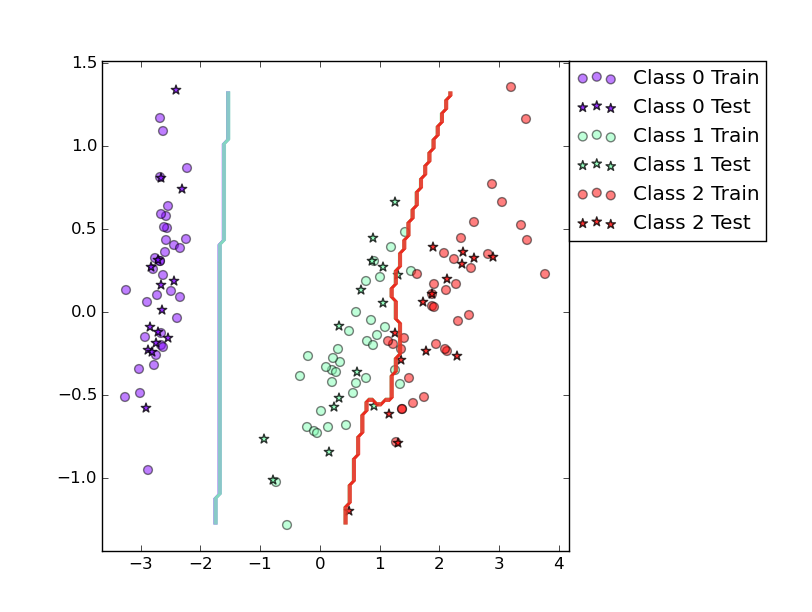
\includegraphics[width = 150mm]{figure_3.png}
  \vspace{-15mm}

  \begin{minipage}[t]{95mm}
    \caption{
      Boundary for the iris data using boosting.
    }
    \label{FIGas3}
  \end{minipage}
\end{figure}
\FloatBarrier

\newpage
\noindent
Questions:
\begin{itemize}
  \item[1)] Is there any improvement in classification accuracy? Why/why not?
  \item[A:] Yes, this is because the boosting puts more weight on the
    missclassified points. This is in accordance with theory, where boosting
    should increase the performance of a high bias low variance classifier
    such as Naive Bayes.
    \marginpar{TODO, har vi koll på detta?}
  \item[2)] Plot the decision boundary of the boosted classifier for the iris set.
    What differences do you notice? Is the boundary of the boosted version more
    complex?
  \item[A:] See Figures \ref{FIGas2} and \ref{FIGas3}. Yes, more complex. Also copes better
    with the correlation
  \item[3)] Can we make up for not using a more complex model by using boosting?
    E.g. not using independent features.
  \item[A:] Yes, at least to some extent.
\end{itemize}



















$ $\\
\textbf{Assignment 6}
\\
Result of running
\begin{scriptsize}
  \begin{verbatim}
  testClassifier(DecisionTreeClassifier(), dataset='iris', split=0.7)
  testClassifier(BoostClassifier(DecisionTreeClassifier(), T=10), dataset='iris',split=0.7)
  testClassifier(DecisionTreeClassifier(), dataset='vowel',split=0.7)
  testClassifier(BoostClassifier(DecisionTreeClassifier(), T=10), dataset='vowel',split=0.7)
  \end{verbatim}
\end{scriptsize}
is given:
\begin{framed}
  \begin{scriptsize}
    \begin{verbatim}
    Trial: 0 Accuracy 95.6
    Trial: 10 Accuracy 100
    Trial: 20 Accuracy 91.1
    Trial: 30 Accuracy 91.1
    Trial: 40 Accuracy 93.3
    Trial: 50 Accuracy 91.1
    Trial: 60 Accuracy 88.9
    Trial: 70 Accuracy 88.9
    Trial: 80 Accuracy 93.3
    Trial: 90 Accuracy 88.9
    Final mean classification accuracy  92.4 with standard deviation 3.71
    Trial: 0 Accuracy 95.6
    Trial: 10 Accuracy 100
    Trial: 20 Accuracy 95.6
    Trial: 30 Accuracy 93.3
    Trial: 40 Accuracy 93.3
    Trial: 50 Accuracy 95.6
    Trial: 60 Accuracy 88.9
    Trial: 70 Accuracy 93.3
    Trial: 80 Accuracy 93.3
    Trial: 90 Accuracy 93.3
    Final mean classification accuracy  94.6 with standard deviation 3.65
    Trial: 0 Accuracy 63.6
    Trial: 10 Accuracy 68.8
    Trial: 20 Accuracy 63.6
    Trial: 30 Accuracy 66.9
    Trial: 40 Accuracy 59.7
    Trial: 50 Accuracy 63
    Trial: 60 Accuracy 59.7
    Trial: 70 Accuracy 68.8
    Trial: 80 Accuracy 59.7
    Trial: 90 Accuracy 68.2
    Final mean classification accuracy  64.1 with standard deviation 4
    Trial: 0 Accuracy 85.7
    Trial: 10 Accuracy 90.3
    Trial: 20 Accuracy 88.3
    Trial: 30 Accuracy 90.9
    Trial: 40 Accuracy 84.4
    Trial: 50 Accuracy 81.2
    Trial: 60 Accuracy 87.7
    Trial: 70 Accuracy 86.4
    Trial: 80 Accuracy 87
    Trial: 90 Accuracy 90.3
    Final mean classification accuracy  86.7 with standard deviation 2.7
    \end{verbatim}
  \end{scriptsize}
\end{framed}





\FloatBarrier
\begin{figure}[h!]
  \center
  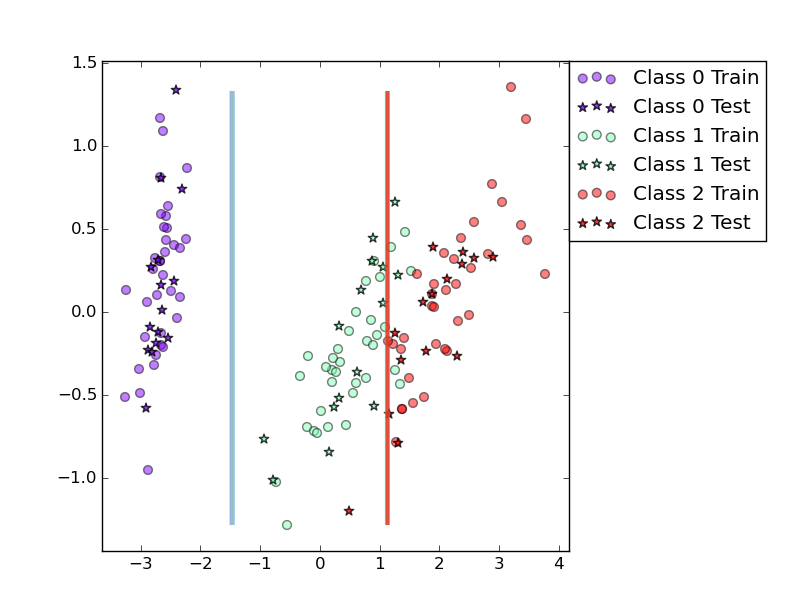
\includegraphics[width = 150mm]{figure_4.png}
  \vspace{-15mm}

  \begin{minipage}[t]{95mm}
    \caption{
      Decision tree.
    }
    \label{FIGas4}
  \end{minipage}
\end{figure}
\FloatBarrier





\FloatBarrier
\begin{figure}[h!]
  \center
  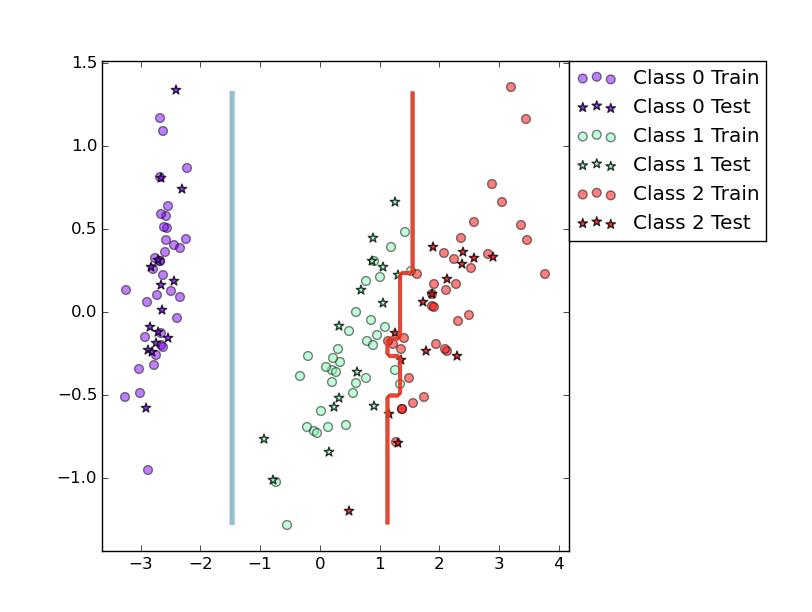
\includegraphics[width = 150mm]{figure_5.png}
  \vspace{-15mm}

  \begin{minipage}[t]{95mm}
    \caption{
      Boosted decision tree.
    }
    \label{FIGas3}
  \end{minipage}
\end{figure}
\FloatBarrier

\newpage
\noindent
Questions:
\begin{itemize}
  \item[1)] Is there any improvement in classification accuracy? Why/why not?
  \item[A:] Yes, in particular for the vowel data set. The mean accuracy increases from
    64.1 \% to 86.7 \%. Not so much for the iris data set. 
    We seem to get accuracy increase from boosting 
    even though decision trees are low bias high variance.
    In theory, bagging should work well for decision trees.
  \item[2)] Plot the decision boundary of the boosted classifier for the iris set.
    What differences do you notice? Is the boundary of the boosted version more
    complex?
  \item[A:] Boosted version is more complex. Both seems to find a boundary that runs
    in parallell to the axes. This is due to splits.
  \item[3)] Can we make up for not using a more complex model by using boosting?
  \item[A:] Yes
\end{itemize}






$ $\\
\textbf{Assignment 7}
\\
If you had to pick a classifier, naive Bayes or a decision tree or
the boosted versions of these, which one would you pick? Motivate from the following
criteria:
\begin{itemize}
  \item Outliers
  \item[-] Naive Bayes with no or little boosting. With boosting, more weight would be put
    on the outliers.
  \item Irrelevant inputs: part of the feature space is irrelevant
  \item[-] Decision tree due to the info-gain feature. With pruning should be good too.
  \item Predictive power
  \item[-] Naive Bayes with boosting
  \item Mixed types of data: binary, categorical or continuous features, etc.
  \item[-] Decision tree should cope well binary, categorical and mixtures of these and 
    continous. Maybe Naive Bayes too if we have suitable probability distributions for the 
    data. Naive Bayes work well with continous data (e.g. image processing).
  \item Scalability: the dimension of the data, D, is large or the number of instances,
    N , is large, or both.
  \item[-] Naive Bayes require moderate or large training set. Decision trees work well when 
    the amount of data increases.
\end{itemize}






\end{document}





